% Mathematical Specification of the Hybrid Triage Engine
% Compile: pdflatex biobert-mathematics.tex (twice)

\documentclass[aspectratio=169,11pt]{beamer}

\usepackage[T1]{fontenc}
\usepackage[utf8]{inputenc}
\usepackage[english]{babel}
\usepackage{lmodern}
\usepackage{amsmath,amssymb,amsfonts}
\usepackage{booktabs}
\usepackage{multicol}
\usepackage{tikz}
\usetikzlibrary{shapes,arrows.meta,positioning,fit,calc}

\usetheme{AnnArbor}
\usecolortheme{wolverine}
\setbeamertemplate{navigation symbols}{}

\definecolor{triageRed}{RGB}{220, 20, 60}
\definecolor{triageOrange}{RGB}{255, 140, 0}
\definecolor{triageYellow}{RGB}{255, 200, 0}
\definecolor{triageGreen}{RGB}{34, 139, 34}

\newcommand{\bcol}[2][blue!70!black]{\textcolor{#1}{#2}}
\newcommand{\why}[1]{\begin{block}{Why we do this}\small #1\end{block}}
\newcommand{\plain}[1]{\begin{block}{In plain English}\small #1\end{block}}

\tikzset{
	flowbox/.style={rectangle, draw=black!60, rounded corners=2pt, fill=blue!8,
		minimum height=0.75cm, align=center, font=\scriptsize, inner sep=3pt},
	flowarr/.style={-{Stealth[length=2mm]}, thick}
}

\title[Hybrid Triage Math Spec]{Mathematics of the Hybrid Triage Engine}
\subtitle{Formulas explained simply --- with diagrams and flowcharts}
\author{Quaigraine Samuel}
\institute{Department of Mathematics\\Kwame Nkrumah University of Science and Technology}
\date{\today}

\begin{document}

\begin{frame}
	\titlepage
\end{frame}

\begin{frame}{Outline}
	\tableofcontents[hideallsubsections]
\end{frame}

% ==================================================================
\section{Big picture}
% ==================================================================

\begin{frame}{What are we building?}
	\plain{Before any formula: a patient describes symptoms (text or voice). The system must output a \textbf{triage colour} (Red / Orange / Yellow / Green) so the hospital knows how urgent the case is.}

	\vspace{0.3em}
	\textbf{Three mathematical helpers work together:}
	\begin{enumerate}
		\item \textbf{BioBERT (NLP)} --- reads words and finds danger signals in language.
		\item \textbf{TEWS (deterministic)} --- adds up points from vital signs (pulse, breathing, etc.).
		\item \textbf{Bayesian (probabilistic)} --- guesses urgency when data are missing or confusing.
	\end{enumerate}

	A \textbf{fusion} step combines all three so no single mistake sends a sick patient to a long wait.
\end{frame}

\begin{frame}{Big picture flowchart}
	\begin{center}
		\resizebox{0.95\textwidth}{!}{%
		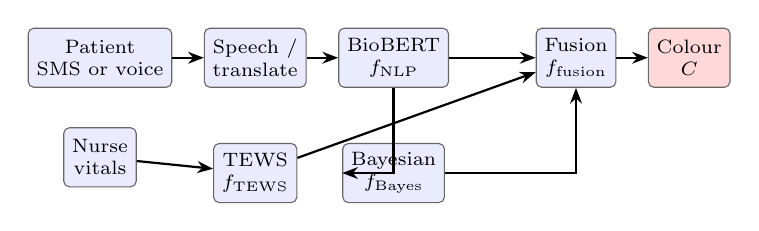
\begin{tikzpicture}[node distance=0.55cm and 0.4cm]
			\node[flowbox] (patient) {Patient\\SMS or voice};
			\node[flowbox, right=of patient] (lang) {Speech /\\translate};
			\node[flowbox, right=of lang] (nlp) {BioBERT\\$f_{\text{NLP}}$};
			\node[flowbox, below=0.7cm of lang] (tews) {TEWS\\$f_{\text{TEWS}}$};
			\node[flowbox, below=0.7cm of nlp] (bayes) {Bayesian\\$f_{\text{Bayes}}$};
			\node[flowbox, right=1.1cm of nlp] (fuse) {Fusion\\$f_{\text{fusion}}$};
			\node[flowbox, right=of fuse, fill=red!15] (out) {Colour\\$C$};
			\node[flowbox, below=0.5cm of patient] (vitals) {Nurse\\vitals};
			\draw[flowarr] (patient) -- (lang);
			\draw[flowarr] (lang) -- (nlp);
			\draw[flowarr] (nlp) -- (fuse);
			\draw[flowarr] (vitals) -- (tews);
			\draw[flowarr] (tews) -- (fuse);
			\draw[flowarr] (nlp.south) |- (bayes.west);
			\draw[flowarr] (bayes.east) -| (fuse.south);
			\draw[flowarr] (fuse) -- (out);
		\end{tikzpicture}}
	\end{center}
	\footnotesize Arrows show \textbf{data flow}. Fusion runs again whenever text or vitals change.
\end{frame}

\begin{frame}{Why three layers instead of one?}
	\begin{columns}[T]
		\column{0.48\textwidth}
		\textbf{If we only use words (NLP):}
		\begin{itemize}
			\item Misses objective physiology
			\item Can misread slang / translation
		\end{itemize}

		\column{0.48\textwidth}
		\textbf{If we only use vitals (TEWS):}
		\begin{itemize}
			\item Fails when patient has no cuff at home
			\item Misses ``crushing chest pain'' with normal pulse
		\end{itemize}
	\end{columns}

	\why{Each layer covers a gap in the others. Mathematics makes the combination \textbf{repeatable} and \textbf{auditable} for a hospital thesis and for clinical governance.}
\end{frame}

% ==================================================================
\section{System formalism}
% ==================================================================

\begin{frame}{Symbols --- plain language first}
	\small
	\begin{tabular}{@{}p{0.22\textwidth}p{0.68\textwidth}@{}}
		\toprule
		\textbf{Symbol} & \textbf{Meaning in simple terms} \\
		\midrule
		$X$ & What the patient said (in English for BioBERT) \\
		$\mathbf{D}$ & How strongly each \textbf{SATS discriminator} appears (0 to 1) \\
		$T$ & TEWS danger score from vitals (a whole number) \\
		$E$ & All evidence: symptoms + any measured vitals \\
		$\mathbf{P}$ & Probability of each colour given $E$ \\
		$C$ & Final colour the patient is sent to \\
		\bottomrule
	\end{tabular}

	\vspace{0.3em}
	Next slides use these symbols in formulas.
\end{frame}

\begin{frame}{Global notation}
	\small
	\begin{tabular}{@{}ll@{}}
		\toprule
		\textbf{Symbol} & \textbf{Meaning} \\
		\midrule
		$s$ & Patient session identifier \\
		$t$ & Event timestamp \\
		$X$ & English-normalised symptom text \\
		$X_{\text{tw}}$ & Optional raw Twi transcript \\
		$\mathbf{D}=(d_1,\ldots,d_m)$ & Discriminator scores, $d_j\in[0,1]$ \\
		$\mathbf{v}=(v_1,\ldots,v_n)$ & Vital-sign vector (SATS parameters) \\
		$T$ & TEWS score, $T\in\mathbb{Z}_{\geq 0}$ \\
		$E$ & Evidence vector (NLP + partial vitals) \\
		$\mathbf{P}$ & Posteriors $P(C_k\mid E)$ over colours $k$ \\
		$C$ & Final pathway colour \\
		$\tau,\tau_B$ & Discriminator / disease override thresholds \\
		\bottomrule
	\end{tabular}
\end{frame}

\begin{frame}{Hybrid session state}
	The engine maintains a session state for each patient $s$:
	\[
	\mathbf{S}_s = \bigl(X,\, \mathbf{D},\, T,\, \mathbf{P},\, C,\, \text{flags}\bigr)
	\]
	\[
	\mathbf{P} = \bigl(P(C_{\text{Red}}\mid E),\, P(C_{\text{Orange}}\mid E),\, P(C_{\text{Yellow}}\mid E),\, P(C_{\text{Green}}\mid E)\bigr)
	\]

	\textbf{Flags:} \texttt{incomplete\_vitals}, \texttt{override\_nlp}, \texttt{override\_bayes}, language code.

	\why{We store everything in $\mathbf{S}_s$ so each module reads the same patient story---like one hospital file that updates as new messages or vitals arrive.}
\end{frame}

\begin{frame}{Three layers as functions}
	\[
	\mathbf{D} = f_{\text{NLP}}(X;\,\theta_{\text{BERT}}),
	\qquad
	T = f_{\text{TEWS}}(\mathbf{v}),
	\qquad
	\mathbf{P} = f_{\text{Bayes}}(E)
	\]
	\[
	C = f_{\text{fusion}}(\mathbf{D},\, T,\, \mathbf{P},\,\text{flags})
	\]

	\vspace{0.4em}
	$f_{\text{NLP}}$: BioBERT encoder + classification head.\\
	$f_{\text{TEWS}}$: piecewise SATS scoring (deterministic).\\
	$f_{\text{Bayes}}$: discrete Bayesian network / table lookup.\\
	$f_{\text{fusion}}$: priority rules (Algorithm 1, later).

	\plain{Think of each $f_{\cdot}$ as a \textbf{function machine}: input goes in, a well-defined output comes out. That is what makes the chatbot testable in a thesis.}
\end{frame}

\begin{frame}{Layer functions flowchart}
	\begin{center}
		\resizebox{0.88\textwidth}{!}{%
		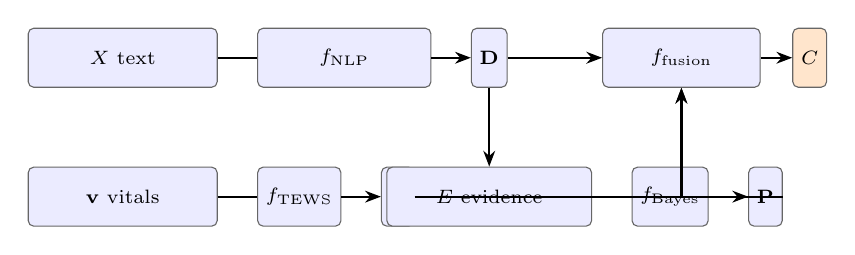
\begin{tikzpicture}[node distance=0.6cm]
			\node[flowbox, minimum width=2.4cm] (x) {$X$ text};
			\node[flowbox, right=0.5cm of x, minimum width=2.2cm] (fnlp) {$f_{\text{NLP}}$};
			\node[flowbox, right=0.5cm of fnlp] (d) {$\mathbf{D}$};
			\node[flowbox, below=1cm of x, minimum width=2.4cm] (v) {$\mathbf{v}$ vitals};
			\node[flowbox, right=0.5cm of v] (ftews) {$f_{\text{TEWS}}$};
			\node[flowbox, right=0.5cm of ftews] (t) {$T$};
			\node[flowbox, below=1cm of d, minimum width=2.6cm] (e) {$E$ evidence};
			\node[flowbox, right=0.5cm of e] (fb) {$f_{\text{Bayes}}$};
			\node[flowbox, right=0.5cm of fb] (p) {$\mathbf{P}$};
			\node[flowbox, right=1.2cm of d, minimum width=2cm] (ff) {$f_{\text{fusion}}$};
			\node[flowbox, right=0.4cm of ff, fill=orange!20] (c) {$C$};
			\draw[flowarr] (x)--(fnlp)--(d);
			\draw[flowarr] (v)--(ftews)--(t);
			\draw[flowarr] (d.south)--(e.north);
			\draw[flowarr] (t.east)-|(ff.south);
			\draw[flowarr] (e)--(fb)--(p);
			\draw[flowarr] (p.east)-|(ff.south);
			\draw[flowarr] (d)--(ff);
			\draw[flowarr] (ff)--(c);
		\end{tikzpicture}}
	\end{center}
\end{frame}

\begin{frame}{Evidence vector construction}
	\[
	E = \mathrm{concat}\bigl(\mathrm{NER}(X),\, \mathbf{v}_{\text{obs}}\bigr)
	\]
	\begin{itemize}
		\item $\mathrm{NER}(X)$: symptom entities and severity tokens from Layer 1
		\item $\mathbf{v}_{\text{obs}}$: subset of vitals with valid measurements
		\item Missing $v_k$ omitted from $E$; flagged for Bayesian imputation
	\end{itemize}

	\why{$E$ is the \textbf{shared language} between NLP and Bayes. Symptoms from text and numbers from vitals are combined so probability math sees the whole picture, not just one modality.}
\end{frame}

\begin{frame}{Execution order and updates}
	\textbf{Parallel (when inputs available):}
	\begin{itemize}
		\item $f_{\text{NLP}}(X)$ on every text/voice-derived message
		\item $f_{\text{Bayes}}(E)$ whenever $E$ changes
	\end{itemize}

	\textbf{Sequential trigger:}
	\begin{itemize}
		\item $f_{\text{TEWS}}(\mathbf{v})$ when nurse enters or updates vitals
		\item $f_{\text{fusion}}$ after \textit{any} update to $\mathbf{D}$, $T$, or $\mathbf{P}$
	\end{itemize}

	\textbf{Re-triage:} $\mathbf{S}_s$ is mutable; $C$ may upgrade (e.g.\ Green $\to$ Orange) without new patient text.
\end{frame}

\begin{frame}{Urgency ordinal scale}
	Define urgency ordinals for fusion safety:
	\[
	\mathrm{ord}(\text{Red})=4,\;
	\mathrm{ord}(\text{Orange})=3,\;
	\mathrm{ord}(\text{Yellow})=2,\;
	\mathrm{ord}(\text{Green})=1
	\]
	\textbf{Safety invariant (configured):}
	\[
	\mathrm{ord}(C) \geq \max\bigl\{\mathrm{ord}(C_{\text{disc}}),\, \mathrm{ord}(C_{\text{TEWS}}),\, \mathrm{ord}(C_{\text{Bayes}})\bigr\}
	\]
	where $C_{\text{disc}}$ is the colour implied by active discriminators in $\mathbf{D}$.
\end{frame}

% ==================================================================
\section{Data requirements}
% ==================================================================

\begin{frame}{Patient and session input data}
	\small
	\begin{tabular}{@{}p{0.32\textwidth}p{0.58\textwidth}@{}}
		\toprule
		\textbf{Field} & \textbf{Type / example} \\
		\midrule
		\texttt{session\_id} & UUID \\
		\texttt{language} & \texttt{en}, \texttt{tw} \\
		\texttt{symptom\_text} or audio & string or blob \\
		\texttt{age}, \texttt{sex} & optional covariates for priors \\
		Self-reported HR, RR & optional $v_k$ (low trust) \\
		\bottomrule
	\end{tabular}

	\textbf{Consumed by:} ASR, translation, $f_{\text{NLP}}$, partial $f_{\text{TEWS}}$.
\end{frame}

\begin{frame}{Clinical and configuration data}
	\small
	\begin{tabular}{@{}p{0.28\textwidth}p{0.32\textwidth}p{0.30\textwidth}@{}}
		\toprule
		\textbf{Category} & \textbf{Examples} & \textbf{Used by} \\
		\midrule
		Nurse vitals & mobility, RR, HR, temp, AVPU, trauma & $f_{\text{TEWS}}$ \\
		SATS tables & $f_k(\cdot)$, $w_k$ & $f_{\text{TEWS}}$ \\
		Discriminator list & $\mathcal{D}_{\text{SATS}}$ labels & NLP head \\
		Bayesian priors & $P(C_k)$, $P(E\mid C_k)$ & $f_{\text{Bayes}}$ \\
		Model weights & BioBERT + classifier $\theta$ & $f_{\text{NLP}}$ \\
		\bottomrule
	\end{tabular}
\end{frame}

\begin{frame}{Audit and governance data}
	Every session must log (immutable append):
	\begin{itemize}
		\item $X_{\text{tw}}$, $X$ (post-translation), ASR confidence
		\item Token-level attention highlights (optional interpretability)
		\item $\mathbf{D}$, $T$, $\mathbf{P}$, $C$ at each fusion step
		\item Timestamp and module version IDs
	\end{itemize}

	\textbf{Purpose:} Clinical review, bias audits, thesis evaluation metrics.

	\why{Without logs you cannot explain \textbf{why} the chatbot chose Orange. For a thesis and for KATH governance, every formula output must be reproducible from stored inputs.}
\end{frame}

\begin{frame}{Training vs runtime data}
	\small
	\begin{tabular}{@{}ll@{}}
		\toprule
		\textbf{Phase} & \textbf{Data} \\
		\midrule
		BioBERT pre-training & PubMed + PMC (external; downloaded weights) \\
		Fine-tuning (optional) & KATH-labelled $(X,\text{discriminator})$ pairs \\
		Bayesian calibration & Historical triage outcomes at hospital \\
		\textbf{Runtime} & Single-session inputs only; no batch retrain \\
		\bottomrule
	\end{tabular}
\end{frame}

\begin{frame}{Minimum viable prototype (FYP)}
	\textbf{Required:} English $X$ + manual vital entry + static SATS tables + fusion code.

	\textbf{Optional modules:} voice ASR, Twi translation, live Bayesian DB.

	\textbf{Cross-reference:} System narrative deck --- \texttt{biobert/integration/hybrid-triage-system.pdf}.
\end{frame}

% ==================================================================
\section{Inter-module interfaces}
% ==================================================================

\begin{frame}{How software modules talk to each other}
	\begin{center}
		\resizebox{0.92\textwidth}{!}{%
		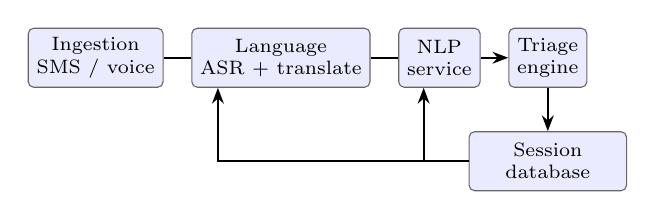
\begin{tikzpicture}[node distance=0.45cm and 0.35cm]
			\node[flowbox] (ing) {Ingestion\\SMS / voice};
			\node[flowbox, right=of ing] (lng) {Language\\ASR + translate};
			\node[flowbox, right=of lng] (nlpm) {NLP\\service};
			\node[flowbox, right=of nlpm] (tri) {Triage\\engine};
			\node[flowbox, below=0.55cm of tri, minimum width=2cm] (db) {Session\\database};
			\draw[flowarr] (ing)--(lng)--(nlpm)--(tri);
			\draw[flowarr] (tri)--(db);
			\draw[flowarr] (db.west)-|([xshift=-0.2cm]nlpm.south);
			\draw[flowarr] (db.west)-|([xshift=-0.8cm]lng.south);
		\end{tikzpicture}}
	\end{center}

	\plain{Modules do not call each other in a tangle---they all read/write one \textbf{session record} in a database. That is how we keep voice, text, and nurse vitals in sync.}
\end{frame}

\begin{frame}[fragile]{Session record schema}
	\footnotesize
	\begin{verbatim}
session_id, language, created_at
transcript_tw, transcript_en, asr_confidence
entities: [{label, span, score}]
discriminators: {d_j: float}
vitals: {v_k: float | null}
TEWS: T, tews_incomplete: bool
posteriors: {C_k: P(C_k|E)}
final_colour: C, fusion_log: [...]
	\end{verbatim}
\end{frame}

\begin{frame}[fragile]{Service API sequence}
	\footnotesize
	\begin{verbatim}
POST /speech/recognize  -> transcript, language_code
POST /translate         -> english_text
POST /nlp/analyze       -> entities, discriminators D
POST /triage/compute    -> TEWS T, posteriors P, colour C
	\end{verbatim}
	Each call reads/writes fields in the session record; \texttt{/triage/compute} runs $f_{\text{fusion}}$.
\end{frame}

\begin{frame}{Invocation timeline}
	\textbf{Phase 1 (pre-hospital):} Patient submits text/voice $\Rightarrow$ $f_{\text{NLP}}$, $f_{\text{Bayes}}$ on partial $E$ $\Rightarrow$ provisional $C$.

	\textbf{Phase 2 (triage desk):} Nurse enters $\mathbf{v}$ $\Rightarrow$ $f_{\text{TEWS}}$ $\Rightarrow$ $f_{\text{fusion}}$ $\Rightarrow$ final $C$.

	\textbf{Phase 3 (optional):} Re-check vitals $\Rightarrow$ update $T$, re-run fusion.
\end{frame}

% ==================================================================
\section{Voice and translation pipeline}
% ==================================================================

\begin{frame}{Voice pipeline flowchart}
	\begin{center}
		\resizebox{0.9\textwidth}{!}{%
		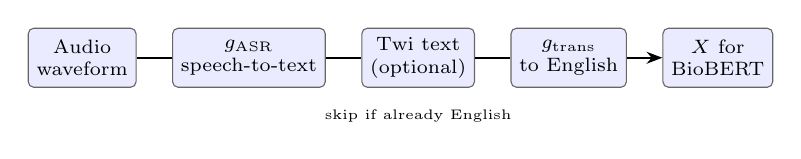
\begin{tikzpicture}[node distance=0.5cm]
			\node[flowbox] (aud) {Audio\\waveform};
			\node[flowbox, right=0.45cm of aud] (asr) {$g_{\text{ASR}}$\\speech-to-text};
			\node[flowbox, right=0.45cm of asr] (twi) {Twi text\\(optional)};
			\node[flowbox, right=0.45cm of twi] (tr) {$g_{\text{trans}}$\\to English};
			\node[flowbox, right=0.45cm of tr] (x) {$X$ for\\BioBERT};
			\draw[flowarr] (aud)--(asr)--(twi)--(tr)--(x);
			\node[below=0.15cm of twi, font=\tiny, align=center] {skip if already English};
		\end{tikzpicture}}
	\end{center}

	\why{BioBERT was trained on biomedical \textbf{English}. Twi must become English first, or we use a glossary fallback $G$ when Google Translation does not support Twi.}
\end{frame}

\begin{frame}{Formal voice-to-text pipeline}
	Let $\mathrm{audio} \in \mathbb{R}^{N}$ be the sampled waveform (numbers describing sound pressure over time).

	\textbf{English path:}
	\[
	X = g_{\text{ASR}}(\mathrm{audio}), \quad \texttt{lang} = \texttt{en}
	\]

	\textbf{Twi path:}
	\[
	X = g_{\text{trans}}\!\bigl(g_{\text{ASR}}(\mathrm{audio})\bigr)
	\]
	Alternatively: $X = G(\tilde{X})$ for glossary fallback $G$ if API unavailable.

	\plain{$g_{\text{ASR}}$ turns sound into letters; $g_{\text{trans}}$ turns Twi letters into English letters BioBERT can understand.}
\end{frame}

\begin{frame}{Google Cloud API parameters}
	\small
	\begin{tabular}{@{}lll@{}}
		\toprule
		\textbf{API} & \textbf{Maps to} & \textbf{Billing} \\
		\midrule
		Speech-to-Text & $g_{\text{ASR}}$ & GCP account; limited free tier \\
		Translation & $g_{\text{trans}}$ & $\sim$500k chars/month free (NMT) \\
		\bottomrule
	\end{tabular}

	\vspace{0.3em}
	\textbf{Twi caveat:} ISO code \texttt{tw} may not be supported on Translation API --- verify at deploy time or use fallback $G$.
\end{frame}

\begin{frame}{Translation error and NLP sensitivity}
	Model input:
	\[
	X = \hat{X} + \epsilon, \quad \epsilon \text{ translation/ASR noise}
	\]

	\textbf{Mitigations:}
	\begin{itemize}
		\item Threshold $\tau$ on $d_j$ before discriminator override
		\item Bayesian $P(C_k\mid E)$ smooths sparse errors
		\item Human audit of $(X_{\text{tw}}, X)$ pairs in pilot
	\end{itemize}
\end{frame}

% ==================================================================
\section{Layer 1: NLP and BioBERT}
% ==================================================================

\begin{frame}{What BioBERT does in one sentence}
	\plain{BioBERT reads the patient's sentence and outputs \textbf{scores} for clinical danger patterns (SATS discriminators), using the same Transformer math as BERT but trained on medical literature.}

	\begin{center}
		\resizebox{0.85\textwidth}{!}{%
		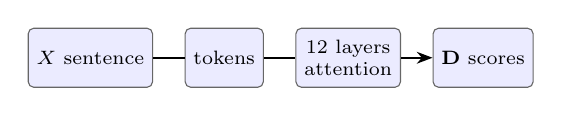
\begin{tikzpicture}[node distance=0.45cm]
			\node[flowbox] (x) {$X$ sentence};
			\node[flowbox, right=0.4cm of x] (tok) {tokens};
			\node[flowbox, right=0.4cm of tok] (enc) {12 layers\\attention};
			\node[flowbox, right=0.4cm of enc] (d) {$\mathbf{D}$ scores};
			\draw[flowarr] (x)--(tok)--(enc)--(d);
		\end{tikzpicture}}
	\end{center}
\end{frame}

\begin{frame}{Tokenisation}
	Given $X = w_1 w_2 \cdots w_L$, WordPiece tokeniser $\tau$ produces
	\[
	\tau(X) = (t_1,\ldots,t_M), \quad M \geq L
	\]
	Special tokens: \texttt{[CLS]} at $t_1$, \texttt{[SEP]} for sentence pairs.

	\textbf{Output dimension:} $M \leq 512$ (BERT max sequence length).

	\why{Computers need discrete tokens, not raw strings. WordPiece splits rare medical words (e.g.\ ``tachycardia'') into pieces the model has seen during training.}
\end{frame}

\begin{frame}{Input embedding}
	For each token $t_i$:
	\[
	E(t_i) = E_{\text{word}}(t_i) + E_{\text{pos}}(i) + E_{\text{seg}}(t_i)
	\]
	Stack into matrix $H^{(0)} \in \mathbb{R}^{M \times d}$ with $d=768$ (BERT-Base).

	\textbf{Contextual:} $E_{\text{word}}$ is a lookup; final $H^{(L)}$ is contextualised by attention.

	\why{We add \textbf{position} so the model knows word order, and \textbf{segment} so it can tell sentence A from sentence B. Without position, ``dog bites man'' and ``man bites dog'' would look the same.}
\end{frame}

\begin{frame}{Mean pooling vs attention pooling}
	\textbf{Mean pooling:}
	\[
	\bar{h} = \frac{1}{M}\sum_{i=1}^{M} h_i^{(L)}
	\]

	\textbf{Additive attention (DAM-style):}
	\[
	a(i) = \frac{\exp(s(h_i;\theta))}{\sum_{j=1}^{M}\exp(s(h_j;\theta))},
	\quad
	h_{\text{att}} = \sum_{i=1}^{M} a(i)\, h_i
	\]
	Clinical example: high $a(i)$ on \textit{chest}, \textit{crushing}; low on \textit{I}, \textit{the}.

	\why{Averaging all words treats ``I'' the same as ``crushing''. Attention learns \textbf{weights} $a(i)$ that sum to 1, so the model focuses on clinically important tokens---exactly what triage nurses do when listening.}
\end{frame}

\begin{frame}{Scaled dot-product attention}
	\[
	\mathrm{Attention}(Q,K,V) = \mathrm{softmax}\!\left(\frac{QK^\top}{\sqrt{d_k}}\right) V
	\]
	\[
	Q = H W^Q,\; K = H W^K,\; V = H W^V
	\]

	Row $i$ of $\mathrm{softmax}(QK^\top/\sqrt{d_k})$ is the attention distribution of token $i$ over all tokens.

	\why{$Q$, $K$, $V$ are learned linear transforms of the same sentence. $QK^\top$ measures \textbf{how related} two words are; softmax turns that into percentages. Dividing by $\sqrt{d_k}$ stops the numbers from exploding (standard Transformer trick).}
\end{frame}

\begin{frame}{Multi-head attention}
	For head $h \in \{1,\ldots,H\}$:
	\[
	\mathrm{head}_h = \mathrm{Attention}(Q_h, K_h, V_h)
	\]
	\[
	\mathrm{MultiHead}(H) = \mathrm{Concat}(\mathrm{head}_1,\ldots,\mathrm{head}_H)\, W^O
	\]

	$BERT$-Base: $H=12$, $d_k = d/H = 64$ per head.

	\why{Multiple heads let the model notice different things at once---grammar in one head, symptom relations in another---then concatenate and mix with $W^O$.}
\end{frame}

\begin{frame}{Encoder layer $l$}
	\[
	Z^{(l)} = \mathrm{LN}\!\left(H^{(l-1)} + \mathrm{MultiHead}(H^{(l-1)})\right)
	\]
	\[
	H^{(l)} = \mathrm{LN}\!\left(Z^{(l)} + \mathrm{FFN}(Z^{(l)})\right)
	\]

	\textbf{FFN (per position):}
	\[
	\mathrm{FFN}(x) = \mathrm{GELU}(x W_1 + b_1) W_2 + b_2
	\]

	$BERT$-Base: $L=12$ identical layers.

	\why{Residual connections ($+H^{l-1}$) let gradients flow through 12 layers during training. LayerNorm keeps values stable. FFN adds non-linear ``thinking'' per word after attention mixes information.}
\end{frame}

\begin{frame}{MLM pre-training objective}
	Masked set $\mathcal{M}$ ($\sim$15\% of tokens):
	\[
	\mathcal{L}_{\text{MLM}} = -\sum_{i \in \mathcal{M}} \log P(t_i \mid H^{(L)};\theta)
	\]

	BioBERT: continue MLM on PubMed/PMC corpora starting from BERT weights $\theta_0 \to \theta_{\text{Bio}}$.

	\why{MLM teaches the model to predict hidden words from context---like fill-in-the-blank on millions of medical sentences. That is how it learns \textbf{meaning}, not memorisation of one patient message.}
\end{frame}

\begin{frame}{Discriminator classification head}
	Let $h_{\texttt{[CLS]}} = H^{(L)}_{1,:}$. For discriminator $j$:
	\[
	d_j = \sigma\!\bigl(w_j^\top h_{\texttt{[CLS]}} + b_j\bigr)
	\quad\text{or}\quad
	\hat{\mathbf{y}} = \mathrm{softmax}(W h_{\texttt{[CLS]}} + \mathbf{b})
	\]

	Mapping: $\hat{\mathbf{y}} \to \mathcal{D}_{\text{SATS}}$ (central chest pain, altered consciousness, \ldots).

	\textbf{Output:} $\mathbf{D} = (d_1,\ldots,d_m)$.

	\why{The \texttt{[CLS]} token is a summary of the whole sentence. We map it to SATS discriminators with sigmoid/softmax so each $d_j$ is a \textbf{confidence}, not a free-text diagnosis (safer for patients).}
\end{frame}

\begin{frame}{NLP forward chain (inference)}
	\[
	X \xrightarrow{\tau} (t_i)
	\xrightarrow{E} H^{(0)}
	\xrightarrow{L\times} H^{(L)}
	\xrightarrow{\text{head}} \mathbf{D}
	\]

	No masking at inference; single forward pass $O(L \cdot M^2 \cdot d)$ per message.
\end{frame}

\begin{frame}{Optional dimensionality reduction}
	If classifier input dimension $d$ is large:
	\[
	z = W_{\text{PCA}}\, h_{\texttt{[CLS]}}, \quad W_{\text{PCA}} \in \mathbb{R}^{r \times d},\; r \ll d
	\]
	Then $\mathbf{D} = \mathrm{softmax}(W' z + b')$. Used only if prototype latency requires it.
\end{frame}

% ==================================================================
\section{Layer 2: Deterministic TEWS}
% ==================================================================

\begin{frame}{TEWS flowchart}
	\begin{center}
		\resizebox{0.88\textwidth}{!}{%
		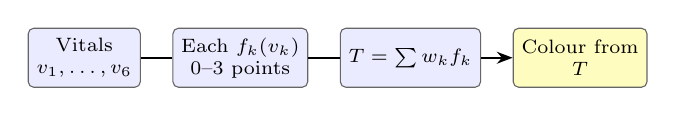
\begin{tikzpicture}[node distance=0.45cm]
			\node[flowbox] (v) {Vitals\\$v_1,\ldots,v_6$};
			\node[flowbox, right=0.4cm of v] (f) {Each $f_k(v_k)$\\0--3 points};
			\node[flowbox, right=0.4cm of f] (sum) {$T=\sum w_k f_k$};
			\node[flowbox, right=0.4cm of sum, fill=yellow!25] (col) {Colour from\\$T$};
			\draw[flowarr] (v)--(f)--(sum)--(col);
		\end{tikzpicture}}
	\end{center}

	\plain{No guessing: same vitals always give the same $T$. That is why hospitals trust TEWS for audits.}
\end{frame}

\begin{frame}{TEWS summation form}
	SATS Triage Early Warning Score:
	\[
	T = f_{\text{TEWS}}(\mathbf{v}) = \sum_{k=1}^{n} w_k\, f_k(v_k)
	\]

	Standard SATS: $w_k = 1$, $n=6$ parameters:
	\begin{enumerate}
		\item Mobility \quad 2. Respiratory rate \quad 3. Heart rate\\
		4. Temperature \quad 5. AVPU \quad 6. Trauma
	\end{enumerate}

	\why{We \textbf{sum} points because SATS defines triage as additive physiology. Each vital is scored independently then added---transparent for nurses and examiners.}
\end{frame}

\begin{frame}{Piecewise score: heart rate $f_1$}
	Example mapping for $v_1 = \mathrm{HR}$ (bpm):
	\[
	f_1(v_1) = \begin{cases}
		3 & v_1 \geq 130 \\
		2 & 111 \leq v_1 \leq 129 \\
		0 & 51 \leq v_1 \leq 100 \\
		2 & v_1 \leq 40 \\
		1 & \text{otherwise (borderline)}
	\end{cases}
	\]

	Each $f_k$ is a \textbf{step function} --- fully deterministic and auditable.

	\why{Step functions encode clinical thresholds (e.g.\ HR $\geq 130$ is dangerous). There is no neural-network randomness---if a nurse disputes a score, you can point to the table.}
\end{frame}

\begin{frame}{Piecewise score: respiratory rate $f_2$}
	For $v_2 = \mathrm{RR}$ (breaths/min), analogous thresholds per SATS manual (e.g.\ RR $\geq 30$ $\Rightarrow$ 3 points).

	\textbf{Numeric example:} $v_1=125 \Rightarrow f_1=2$; $v_2=26 \Rightarrow f_2=2$.
\end{frame}

\begin{frame}{Colour map $C_{\text{TEWS}}(T)$}
	\[
	C_{\text{TEWS}}(T) = \begin{cases}
		\bcol[triageRed]{\text{Red}} & T > 7 \\
		\bcol[triageOrange]{\text{Orange}} & 5 \leq T \leq 6 \\
		\bcol[triageYellow]{\text{Yellow}} & 3 \leq T \leq 4 \\
		\bcol[triageGreen]{\text{Green}} & T \leq 2
	\end{cases}
	\]

	\textbf{Example:} $f_1=2$, $f_2=2$, others $=0$ $\Rightarrow$ $T=4$ $\Rightarrow$ Yellow.
\end{frame}

\begin{frame}{Incomplete vitals}
	Let $\mathcal{K}_{\text{obs}} = \{k : v_k \text{ measured}\}$.

	\textbf{Partial sum:}
	\[
	T_{\text{partial}} = \sum_{k \in \mathcal{K}_{\text{obs}}} w_k f_k(v_k)
	\]

	Set \texttt{tews\_incomplete}$=true$ if $\mathcal{K}_{\text{obs}} \neq \{1,\ldots,n\}$.

	Fusion must not assign Green on $T_{\text{partial}}$ alone when flags indicate missing critical vitals.
\end{frame}

\begin{frame}{TEWS data contract}
	\textbf{Input:} \texttt{vitals} map $\{k: v_k\}$ validated against clinical ranges.

	\textbf{Output:} \texttt{TEWS} $=T$, \texttt{tews\_incomplete}, \texttt{colour\_tews} $= C_{\text{TEWS}}(T)$.

	\textbf{Consumer:} $f_{\text{fusion}}$; also feeds $E$ for $f_{\text{Bayes}}$.
\end{frame}

% ==================================================================
\section{Layer 3: Bayesian model}
% ==================================================================

\begin{frame}{Bayesian layer flowchart}
	\begin{center}
		\resizebox{0.85\textwidth}{!}{%
		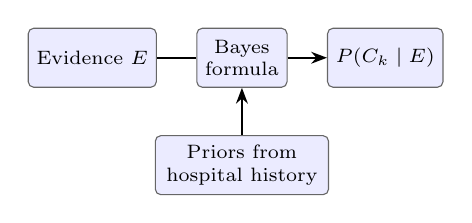
\begin{tikzpicture}[node distance=0.45cm]
			\node[flowbox] (e) {Evidence $E$};
			\node[flowbox, right=0.5cm of e] (bay) {Bayes\\formula};
			\node[flowbox, right=0.5cm of bay] (p) {$P(C_k\mid E)$};
			\node[flowbox, below=0.6cm of bay, minimum width=2.2cm] (prior) {Priors from\\hospital history};
			\draw[flowarr] (e)--(bay)--(p);
			\draw[flowarr] (prior)--(bay);
		\end{tikzpicture}}
	\end{center}

	\plain{When temperature or BP is missing, we still ask: ``Given what we \textit{do} know, which colour is most likely?''}
\end{frame}

\begin{frame}{Colour posterior}
	\[
	P(C_k \mid E) = \frac{P(E \mid C_k)\, P(C_k)}{\sum_{j} P(E \mid C_j)\, P(C_j)}
	\]

	$C_k \in \{\text{Red}, \text{Orange}, \text{Yellow}, \text{Green}\}$.

	$P(C_k)$: hospital prior acuity rates; $P(E\mid C_k)$: likelihood tables from historical data or expert elicitation.

	\why{This is Bayes' rule: \textbf{prior} (how common each urgency is) updated by \textbf{likelihood} (how often we see these symptoms for that urgency). The denominator normalises so probabilities sum to 1.}
\end{frame}

\begin{frame}{Disease-level posterior (override)}
	For latent severe disease $D$ (e.g.\ septic shock, MI) and symptom set $S$ from NLP:
	\[
	P(D \mid S) = \frac{P(S \mid D)\, P(D)}{P(S)}
	\]

	\textbf{Override:} if $P(D\mid S) > \tau_B$ then set $C_{\text{Bayes}} = \text{Red}$ (or Orange per protocol).
\end{frame}

\begin{frame}{Evidence from NLP and vitals}
	\[
	E = \bigl[\text{entity}_1,\ldots,\text{entity}_r,\, v_{k_1},\ldots,v_{k_s}\bigr]
	\]

	Bayesian network structure (conceptual):
	\begin{itemize}
		\item Nodes: $C_k$, key symptoms, optional vital nodes
		\item Missing vital node $\Rightarrow$ marginalise or use prior $P(v_k\mid C_k)$
	\end{itemize}
\end{frame}

\begin{frame}{Incomplete evidence branch}
	When \texttt{tews\_incomplete} or sparse $E$:
	\[
	C_{\text{Bayes}} = \arg\max_{k} P(C_k \mid E)
	\]

	This is the branch used in Algorithm 1 step 5 instead of default Green.
\end{frame}

\begin{frame}{Bayesian data contract}
	\textbf{Input:} $E$, prior tables $P(C_k)$, $P(E\mid C_k)$ or $P(S\mid D)$, $P(D)$.

	\textbf{Output:} $\mathbf{P}$, \texttt{override\_bayes}, optional $P(D\mid S)$.

	\textbf{Static data file:} \texttt{priors\_kath.json} (calibrated offline).
\end{frame}

% ==================================================================
\section{Master fusion controller}
% ==================================================================

\begin{frame}{Fusion decision flowchart}
	\begin{center}
		\resizebox{0.95\textwidth}{!}{%
		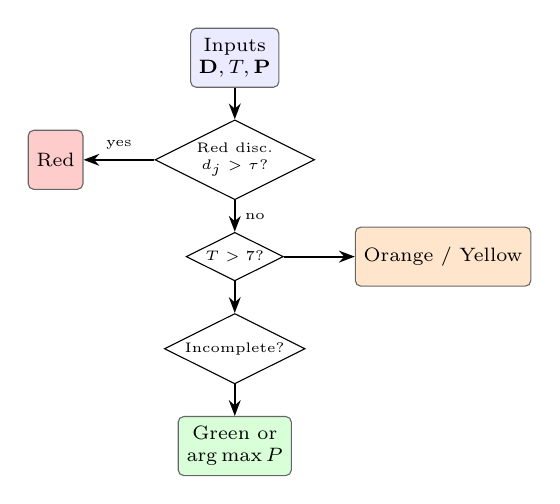
\begin{tikzpicture}[
			node distance=0.35cm and 0.25cm,
			decision/.style={diamond, draw, aspect=2, inner sep=1pt, font=\tiny, align=center}
		]
			\node[flowbox] (start) {Inputs\\$\mathbf{D},T,\mathbf{P}$};
			\node[decision, below=0.4cm of start] (d1) {Red disc.\\$d_j>\tau$?};
			\node[flowbox, left=0.9cm of d1, fill=red!20] (red) {Red};
			\node[decision, below=0.4cm of d1] (t1) {$T>7$?};
			\node[flowbox, right=0.9cm of t1, fill=orange!20] (ora) {Orange / Yellow};
			\node[decision, below=0.4cm of t1] (inc) {Incomplete?};
			\node[flowbox, below=0.4cm of inc, fill=green!15] (gr) {Green or\\$\arg\max P$};
			\draw[flowarr] (start)--(d1);
			\draw[flowarr] (d1)--node[above,font=\tiny]{yes}(red);
			\draw[flowarr] (d1)--node[right,font=\tiny]{no}(t1);
			\draw[flowarr] (t1)--(ora);
			\draw[flowarr] (t1)--(inc);
			\draw[flowarr] (inc)--(gr);
		\end{tikzpicture}}
	\end{center}

	\why{Rules are checked in \textbf{urgency order}. Text can override a low TEWS when SATS says the symptom is inherently dangerous (e.g.\ central chest pain).}
\end{frame}

\begin{frame}{Algorithm 1: Colour assignment}
	\small
	\textbf{Input:} $\mathbf{D}$, $T$, $\mathbf{P}$, flags, thresholds $\tau$, $\tau_B$.

	\begin{enumerate}
		\item If $\exists j: d_j > \tau \land j \in \mathcal{D}_{\text{Red}} \Rightarrow C=\text{Red}$.
		\item Else if $\exists j: d_j > \tau \land j \in \mathcal{D}_{\text{Orange}} \Rightarrow C=\text{Orange}$.
		\item Else if $T > 7 \Rightarrow C=\text{Red}$.
		\item Else if $5 \leq T \leq 6 \Rightarrow C=\text{Orange}$.
		\item Else if $3 \leq T \leq 4 \Rightarrow C=\text{Yellow}$.
		\item Else if \texttt{incomplete} $\Rightarrow C = \arg\max_k P(C_k\mid E)$.
		\item Else if $P(D\mid S) > \tau_B \Rightarrow C=\text{Red}$ (or protocol colour).
		\item Else $C=\text{Green}$.
	\end{enumerate}
\end{frame}

\begin{frame}{Conflict resolution}
	\small
	\begin{center}
		\begin{tabular}{@{}ccc@{}}
			\toprule
			$\mathbf{D}$ & $T$ & \textbf{Result} \\
			\midrule
			High (chest pain) & 4 (Yellow) & Orange (discriminator) \\
			Low & $\geq 7$ & Red (TEWS) \\
			Ambiguous & incomplete & $\arg\max P(C_k\mid E)$ \\
			Low & low & Green \\
			\bottomrule
		\end{tabular}
	\end{center}

	Discriminator and TEWS disagree $\Rightarrow$ take \textbf{more urgent} per $\mathrm{ord}(\cdot)$.
\end{frame}

\begin{frame}{Fusion output contract}
	\textbf{Output to patient:} $C$, wait guidance, safety message.

	\textbf{Output to hospital:} $C$, $\mathbf{D}$, $T$, $\mathbf{P}$, full \texttt{fusion\_log} with rule ID fired (e.g.\ \texttt{RULE\_DISC\_ORANGE}).

	\[
	f_{\text{fusion}}: (\mathbf{D}, T, \mathbf{P}, \text{flags}) \mapsto (C,\; \text{log})
	\]
\end{frame}

\begin{frame}{Module dependency graph (summary)}
	\footnotesize
	$g_{\text{ASR}}, g_{\text{trans}} \to X \to f_{\text{NLP}} \to \mathbf{D}$\\
	$\mathbf{v} \to f_{\text{TEWS}} \to T$\\
	$(\mathbf{D}, \mathbf{v}) \to E \to f_{\text{Bayes}} \to \mathbf{P}$\\
	$(\mathbf{D}, T, \mathbf{P}) \to f_{\text{fusion}} \to C$

	All modules communicate only through the \textbf{session record} schema.
\end{frame}

% ==================================================================
\section{End-to-end numeric trace}
% ==================================================================

\begin{frame}{End-to-end trace flowchart}
	\begin{center}
		\resizebox{0.92\textwidth}{!}{%
		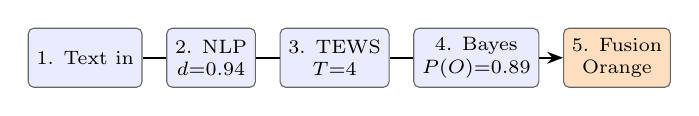
\begin{tikzpicture}[node distance=0.35cm]
			\node[flowbox] (s1) {1. Text in};
			\node[flowbox, right=0.3cm of s1] (s2) {2. NLP\\$d{=}0.94$};
			\node[flowbox, right=0.3cm of s2] (s3) {3. TEWS\\$T{=}4$};
			\node[flowbox, right=0.3cm of s3] (s4) {4. Bayes\\$P(O){=}0.89$};
			\node[flowbox, right=0.3cm of s4, fill=orange!25] (s5) {5. Fusion\\Orange};
			\draw[flowarr] (s1)--(s2)--(s3)--(s4)--(s5);
		\end{tikzpicture}}
	\end{center}
	\footnotesize Follow the numbers on the next slides for the chest-pain example.
\end{frame}

\begin{frame}{Trace setup (English SMS)}
	\textbf{Input $X$:} ``Chest is crushing. Dizzy. Pulse about 125. Breathing 26 per minute. No thermometer.''

	\textbf{Session:} \texttt{lang=en}; vitals from text + nurse pending temp/BP.

	Goal: compute $\mathbf{D}$, $T$, $\mathbf{P}$, $C$ step by step.
\end{frame}

\begin{frame}{Trace: Layer 1 (NLP)}
	Token attention $\alpha_i$: peaks on \textit{crushing}, \textit{chest}, \textit{dizzy}.

	\[
	d_{\text{central\_chest\_pain}} = 0.94,\quad
	d_{\text{other}} \ll \tau
	\]

	Entities: chest pain (severe), dizziness, tachycardia (self-report), tachypnoea.

	$\Rightarrow$ $\mathbf{D}$ triggers discriminator path; $E$ enriched for Bayes.
\end{frame}

\begin{frame}{Trace: Layer 2 (TEWS)}
	From message + nurse: $v_1=\mathrm{HR}=125$, $v_2=\mathrm{RR}=26$.

	\[
	f_1(125)=2,\quad f_2(26)=2,\quad f_{3:6}=0
	\Rightarrow T = 4
	\]

	\[
	C_{\text{TEWS}}(4) = \text{Yellow}
\]

	\texttt{tews\_incomplete}$=$true (temperature, BP missing).
\end{frame}

\begin{frame}{Trace: Layer 3 (Bayesian)}
	$E = \{\text{chest pain}, \text{dizzy}, \mathrm{HR}{=}125, \mathrm{RR}{=}26\}$.

	\[
	P(C_{\text{Orange}} \mid E) \approx 0.89,\quad
	P(C_{\text{Yellow}} \mid E) \approx 0.08
\]

	$P(\mathrm{MI}\mid S)$ elevated due to symptom cluster.
\end{frame}

\begin{frame}{Trace: Fusion result}
	Algorithm 1: step 2 fires ($d_{\text{chest}} > \tau$, Orange discriminator).

	\[
	C = \textbf{Orange},\quad \mathrm{ord}(C)=3 > \mathrm{ord}(C_{\text{TEWS}}(4))=2
\]

	\textbf{Hospital action:} cardiology alert; bypass Green/Yellow queue despite $T=4$.

	\plain{TEWS alone said Yellow ($T=4$), but the \textbf{discriminator} from language said chest pain is an Orange-level SATS finding. Fusion picks the safer, more urgent path.}
\end{frame}

\begin{frame}{Trace: Twi voice path}
	\textbf{Audio} $\to g_{\text{ASR}} \to X_{\text{tw}}$ $\to g_{\text{trans}} \to X$:

	\small\textit{``I have fever, chest hurts, short of breath.''}

	Same chain: $\tau(X) \to H^{(L)} \to \mathbf{D}$; fever + chest + dyspnoea $\Rightarrow$ high cardio-respiratory scores.

	Fusion identical in structure; log $(X_{\text{tw}}, X)$ for audit.
\end{frame}

% ==================================================================
\section{References}
% ==================================================================

\begin{frame}{References}
	\footnotesize
	\begin{itemize}
		\item Vaswani, A., et al.\ (2017). Attention is all you need. \textit{NeurIPS}.
		\item Devlin, J., et al.\ (2018). BERT. arXiv:1810.04805.
		\item Lee, J., et al.\ (2020). BioBERT. \textit{Bioinformatics}, 36(4), 1234--1240.
		\item Gligorijevi\'c, D., et al.\ (2018). Deep attention triage. arXiv:1804.03240.
		\item Stewart, J., et al.\ (2023). NLP at ED triage. \textit{PLoS ONE}, 18(12):e0279953.
		\item SATS Manual (2012); Rominski et al.\ KATH validation.
		\item Google Cloud Speech-to-Text and Translation API documentation.
		\item Project: \texttt{latex/literature-review/lit.tex}, \texttt{latex/nlp-short/nlp.tex}.
	\end{itemize}
\end{frame}

\end{document}
